\newpage
\section{Anhang}
\label{sec:Anhang}

\begin{figure}
  \centering
  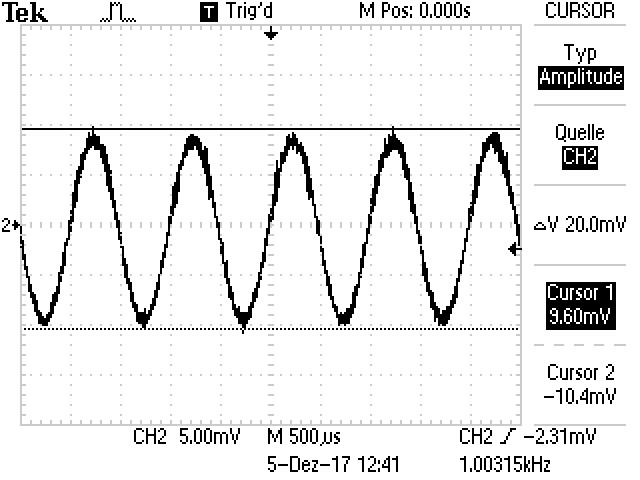
\includegraphics[width=9cm]{data/reference_output.jpg}
  \caption{Ein Signal aus dem Reference Output}
  \label{fig:reference_output}
\end{figure}

\begin{figure}
  \centering
  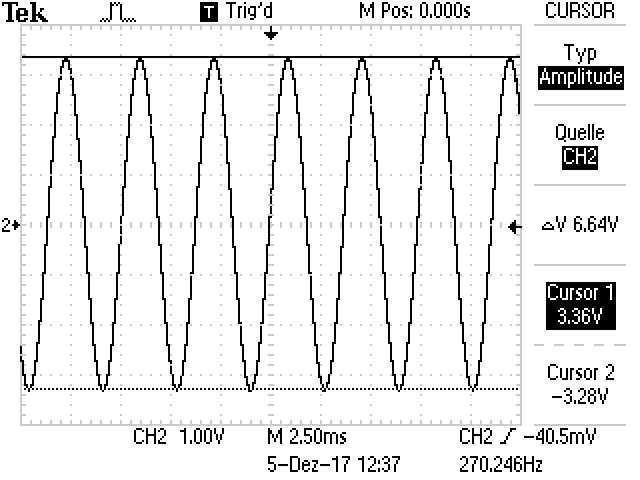
\includegraphics[width=9cm]{data/oscillator_output.jpg}
  \caption{Ein Signal aus dem Oscillator Output}
  \label{fig:oscillator_output}
\end{figure}



\begin{figure}
  \centering
  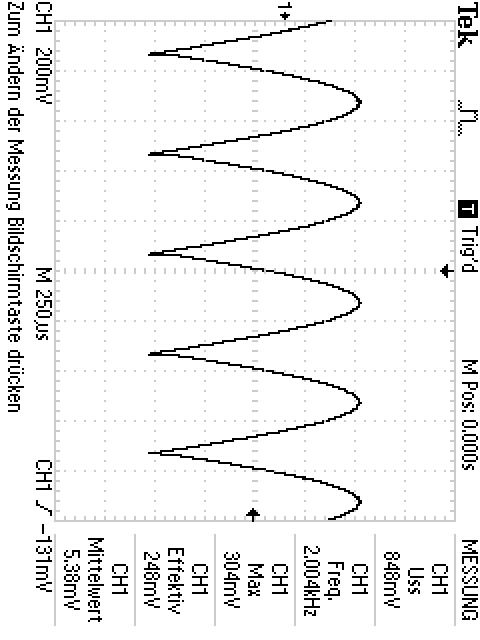
\includegraphics[width=11cm]{data/phase_0.jpg}
  \caption{Ausgangsspannung $U_{\symup{out}}$ bei einer Phasenverschiebung
  von $\phi=0$}
  \label{fig:phase_0}
\end{figure}

\begin{figure}
  \centering
  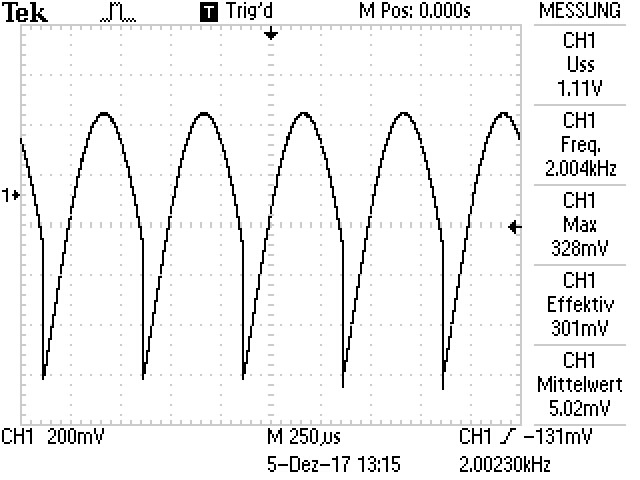
\includegraphics[width=11cm]{data/phase_30.jpg}
  \caption{Ausgangsspannung $U_{\symup{out}}$ bei einer Phasenverschiebung
  von $\phi=\frac{\pi}{6}$}
  \label{fig:phase_30}
\end{figure}

\begin{figure}
  \centering
  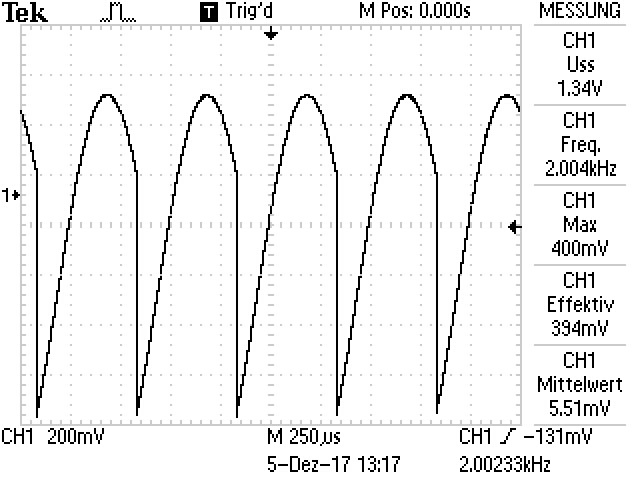
\includegraphics[width=11cm]{data/phase_45.jpg}
  \caption{Ausgangsspannung $U_{\symup{out}}$ bei einer Phasenverschiebung
  von $\phi=\frac{\pi}{4}$}
  \label{fig:phase_45}
\end{figure}

\begin{figure}
  \centering
  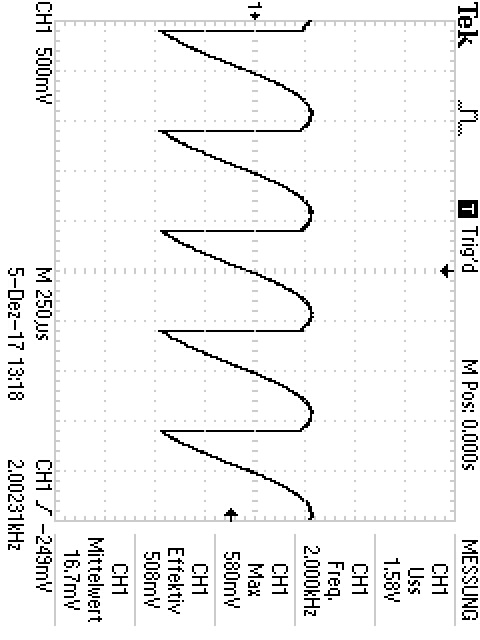
\includegraphics[width=11cm]{data/phase_60.jpg}
  \caption{Ausgangsspannung $U_{\symup{out}}$ bei einer Phasenverschiebung
  von $\phi=\frac{\pi}{3}$}
  \label{fig:phase_60}
\end{figure}

\begin{figure}
  \centering
  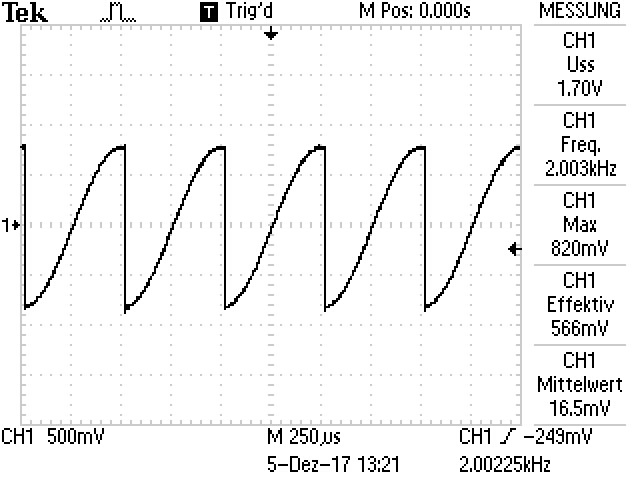
\includegraphics[width=11cm]{data/phase_90.jpg}
  \caption{Ausgangsspannung $U_{\symup{out}}$ bei einer Phasenverschiebung
  von $\phi=\frac{\pi}{2}$}
  \label{fig:phase_0}
\end{figure}





\begin{figure}
  \centering
  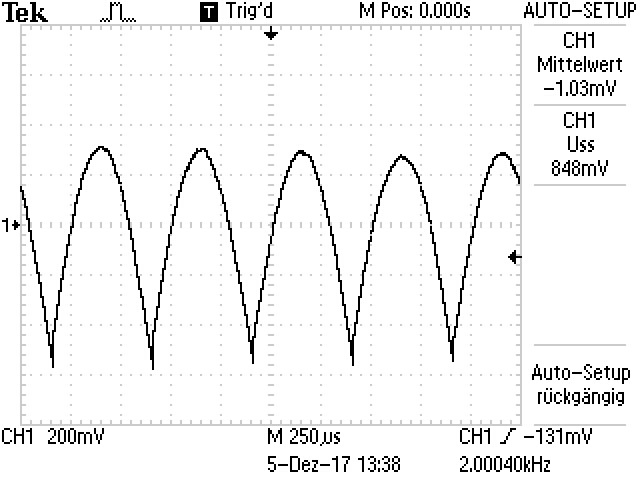
\includegraphics[width=11cm]{data/rauschen_0.jpg}
  \caption{Ausgangsspannung $U_{\symup{out}}$ bei einer Phasenverschiebung
  von $\phi=0$}
  \label{fig:rauschen_0}
\end{figure}

\begin{figure}
  \centering
  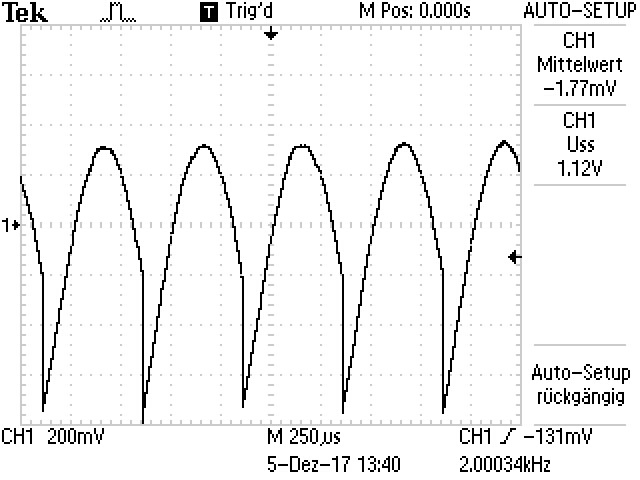
\includegraphics[width=11cm]{data/rauschen_30.jpg}
  \caption{Ausgangsspannung $U_{\symup{out}}$ bei einer Phasenverschiebung
  von $\phi=\frac{\pi}{6}$}
  \label{fig:phase_30}
\end{figure}

\begin{figure}
  \centering
  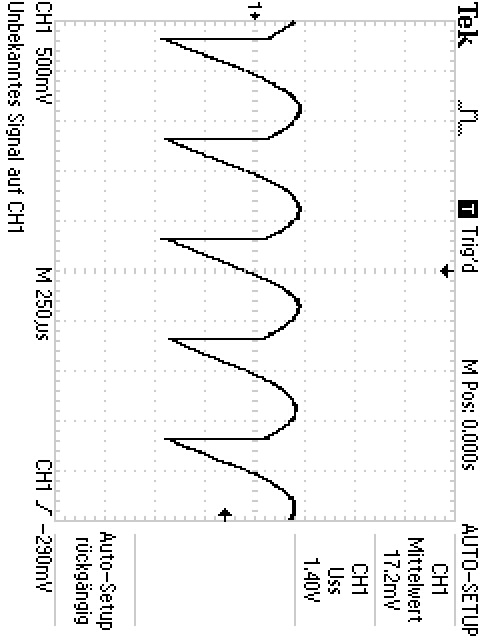
\includegraphics[width=11cm]{data/rauschen_45.jpg}
  \caption{Ausgangsspannung $U_{\symup{out}}$ bei einer Phasenverschiebung
  von $\phi=\frac{\pi}{4}$}
  \label{fig:phase_45}
\end{figure}

\begin{figure}
  \centering
  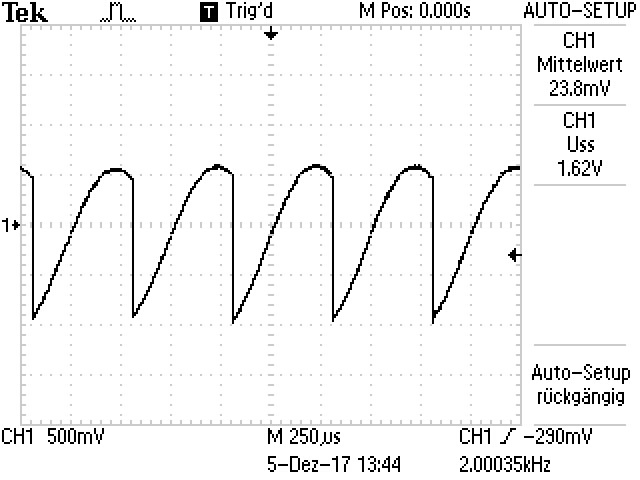
\includegraphics[width=11cm]{data/rauschen_60.jpg}
  \caption{Ausgangsspannung $U_{\symup{out}}$ bei einer Phasenverschiebung
  von $\phi=\frac{\pi}{3}$}
  \label{fig:phase_60}
\end{figure}

\begin{figure}
  \centering
  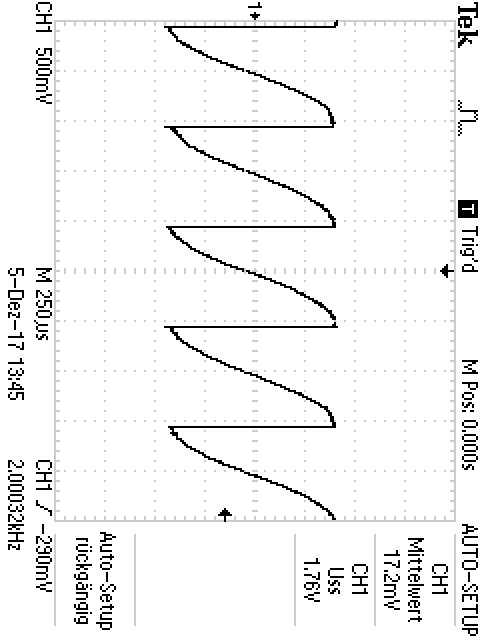
\includegraphics[width=11cm]{data/rauschen_90.jpg}
  \caption{Ausgangsspannung $U_{\symup{out}}$ bei einer Phasenverschiebung
  von $\phi=\frac{\pi}{2}$}
  \label{fig:phase_90}
\end{figure}
